\begin{frame}
    \vspace{-1cm}
    \centering
    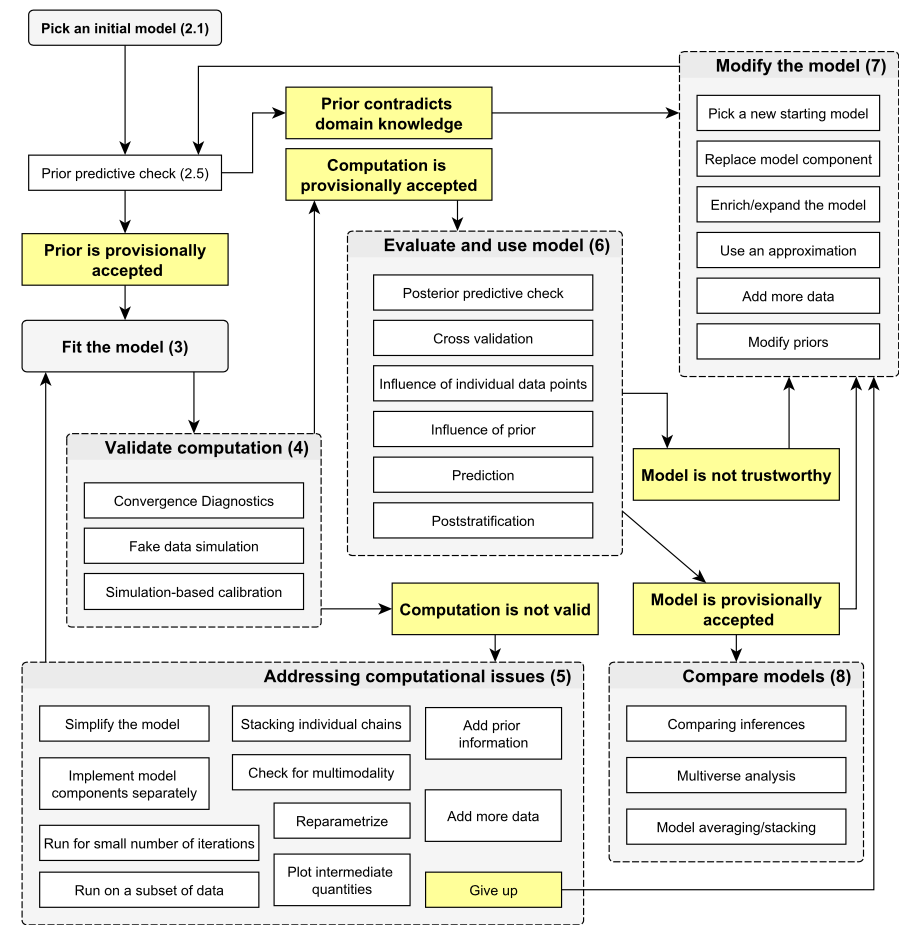
\includegraphics[width=0.75\linewidth]{../graphics/workflow}
\end{frame}

\begin{frame}{Initial model 1: Log-shift transformation}
    Like the model from Morelli, but with full Bayesian inference on the shift term
    \begin{equation}
        \begin{split}
            p(y^*|\boldsymbol \beta, u_d, \sigma_e, \nu)   =        \text{Student}&(\log(y_{di} + \lambda)| \boldsymbol{x'}_{di} \boldsymbol \beta + u_d,\ \sigma_e\ , \nu)\cdot \frac 1 {(y_{di} + \lambda)}, \\
            u_d | \sigma_u & \sim \mathcal N(0, \sigma_u),\ d = 1, ..., D \\
            \beta_k & \sim \mathcal N(\mu_k, \sigma_k),\ k = 1, ..., K\\
            \sigma_u & \sim Ga(2, 0.75), \\
            \sigma_e & \sim Ga(2, 0.75), \\
            \nu & \sim Ga(2, 0.1), \\
            S(y^*) & \sim \mathcal N(0, 0.01),\\
        \end{split}
        \label{eq:trafo_hb}
    \end{equation}
\end{frame}

\begin{frame}{Initial model 1: Tightness of the prior on skewness}

    \begin{columns}
        \begin{column}{0.32\textwidth}
            \includegraphics[width=\linewidth]{../graphics/log_shift/bad_skewness}

            $S(y^*) \sim \mathcal N (0, 0.1)$
        \end{column}



        \begin{column}{0.32\textwidth}
            \includegraphics[width=\linewidth]{../graphics/log_shift/mid_skewness}

            $S(y^*) \sim \mathcal N (0, 0.01)$
        \end{column}


        \begin{column}{0.32\textwidth}
            \includegraphics[width=\linewidth]{../graphics/log_shift/gb2_skewness}

            $S(y^*) \sim \mathcal N (0, 0.001)$
        \end{column}

    \end{columns}
    \vspace{1cm}
    \textbf{Too wide}: unrealistic values and computational problems
    \vspace{0.5cm}

    \textbf{Too tight}: overfitting
\end{frame}

\begin{frame}
    \vspace{-0.5cm}
    \centering
    \includegraphics[width=0.85\linewidth]{../graphics/log_shift/logscale_smp_}

    \scriptsize{Posterior predictive check for log-scale scenario}

    \includegraphics[width=0.85\linewidth]{../graphics/log_shift/gb2_smp_}

    \scriptsize{Posterior predictive check for GB2 scenario}

    \includegraphics[width=0.85\linewidth]{../graphics/log_shift/pareto_smp_}

    \scriptsize{Posterior predictive check for Pareto scenario}

\end{frame}

\begin{frame}{Initial model 2: Skewed likelihoods}
    As an alternative model with skewed likelihoods were estimated:
    \begin{itemize}
        \item Skew-normal
        \item exGaussian
        \item Lognormal
        \item Gamma (log link)
        \item Gamma (softplus link)
    \end{itemize}
\end{frame}

\begin{frame}{Initial model 2: Skewed likelihoods}
    Additive likelihoods did not work well in the log-scale scenario

    \begin{columns}
        \begin{column}{0.49\textwidth}
            \centering
            \includegraphics[width=\linewidth]{../graphics/skewed_likelihood/single_graphs/skewnormal_logscale}

            Skew-normal
        \end{column}

        \begin{column}{0.49\textwidth}
            \centering
            \includegraphics[width=\linewidth]{../graphics/skewed_likelihood/single_graphs/exgaussian_logscale}

            exGaussian
        \end{column}
    \end{columns}

\end{frame}

\begin{frame}
    \vspace{-0.5cm}
    \scriptsize{The gamma log link had the best results of all the skewed likelihoods}
    \centering
    \includegraphics[width=0.8\linewidth]{../graphics/skewed_likelihood/gamma_log/logscale_smp_gamma_log}

    \scriptsize{Posterior predictive check for log-scale scenario}

    \includegraphics[width=0.8\linewidth]{../graphics/skewed_likelihood/gamma_log/gb2_smp_gamma_log}

    \scriptsize{Posterior predictive check for GB2 scenario}

    \includegraphics[width=0.8\linewidth]{../graphics/skewed_likelihood/gamma_log/pareto_smp_gamma_log}

    \scriptsize{Posterior predictive check for Pareto scenario}

\end{frame}

\begin{frame}{Defining priors on coefficients}
    \begin{itemize}
        \item In the log-shift model, coefficient are approximately percentage changes
        \item A change of more than 30\% for an additional unit seems excessive
        \item Coefficient prior is set to $\beta_k \sim \mathcal N(0, 0.2)$
    \end{itemize}
\end{frame}

\begin{frame}{Defining priors on scale parameters}
    \begin{itemize}
        \item $\sigma_e$ is not the standard deviation for a Student distribution
        \item The variance is defined as $\sigma^2 = \sigma_e^2\frac {\nu} {\nu -2}$
        \item $\sigma_e$ is redefined as $\sigma_e = \sigma \sqrt{\frac{\nu -2}{\nu}}$
        \item The gamma prior $Ga(2, a)$ is now placed on $\sigma_u$ and $\sigma$
        \item The rate parameter $a$ is determined with prior predictive checks
    \end{itemize}
\end{frame}

\begin{frame}{Prior predictive checks: scale prior}

    \centering
    Original scale prior: $Ga(2, 0.75)$
    \includegraphics[width=0.8\linewidth]{../graphics/prior_predictive_checks/prior_check_gb2_start}
\end{frame}

\begin{frame}{Prior predictive checks: scale prior}
    \centering
    Tight scale prior: $Ga(2, 7)$
    \includegraphics[width=0.8\linewidth]{../graphics/prior_predictive_checks/prior_check_gb2_wide}
\end{frame}

\begin{frame}{Prior predictive checks: scale prior}
    \centering
    Tight scale prior: $Ga(2, 0.7)$
    \includegraphics[width=0.8\linewidth]{../graphics/prior_predictive_checks/prior_check_gb2_tight}
\end{frame}